\section{Methods}\label{sec:method}
\section{Problem Formulation}\label{sec:problem}
A policy receives camera images, proprioception, and instruction $\ell$, and predicts an action chunk. The controller executes a prefix before replanning. Let $h_t$ denote the available observation history and $c$ the scene initialization. We optimize binary complete-task success $Y(\tau)$:
\begin{equation}
J(\theta)=\mathbb E_{(c,\ell)\sim\rho_{\rm full},\,\tau\sim P_\theta(\cdot\mid c,\ell)}[Y(\tau)].
\end{equation}
Individual skills have their own instructions, success predicates, and reset distributions $\rho_k$. Placement from a held-object start is therefore a skill test, not full pick-and-place. A training stage is a step in the learning schedule; a task phase is progress within an episode.

The CDPR action has five channels: Cartesian translation, yaw, and gripper control. Strict success requires grasp, held lift, intentional release, and native placement, without carry-slip or wrong-placement events. LIBERO uses its native goal verifier~\cite{libero}. We report these different evaluation settings separately.


\subsection{Dense Acquisition, Binary Refinement, and Self-Imitation}
We first train approach, pickup, and placement skills with dense rewards. Distance reduction and manipulation events guide exploration before skill success becomes common. After dense acquisition, we refine the skills using binary success rewards.

Successful trajectories are retained by instruction. When later training degrades earlier skills, self-imitation fits a balanced mixture of earlier and current successes:
\begin{equation}
\mathcal L_{\rm SI}=\mathbb E_{\rm success}
\left[\|\hat a-a\|^2\right].
\label{eq:si_loss}
\end{equation}
Here $\hat a$ is the predicted action and $a$ is the recorded executed action. The average balances instructions and excludes unused action slots. Policy-dependent features are refreshed before fitting. Balancing matters because imitating only the newest skill can reinforce forgetting.

Algorithm~\ref{alg:paper_pipeline} summarizes the schedule. Progress is checked with fixed skill evaluations. After an initial training period, automated stages can end at a success target or a plateau; budget exhaustion also ends a stage. The CDPR sequence used validation-guided manual transitions. After consolidation, all learned skills are evaluated again. Automated runs retain the consolidation update only when recovery improves the degraded skills on average and keeps other skills within tolerance.
% Method-level schedule. Automatic stopping is implemented for WX200;
% the historical CDPR sequence used validation-guided manual transitions.
\begin{algorithm}[!t]
\caption{Staged VLA adaptation}
\label{alg:paper_pipeline}
\small
\begin{algorithmic}[1]
\Require Pretrained VLA, skill instructions, fixed evaluations
\State Initialize the target action controller and success banks
\For{reward mode: dense acquisition, then binary refinement}
    \For{skill: approach, pickup, placement}
        \Repeat
            \State Collect same-scene rollout groups for the skill
            \State Update with $\mathcal L_{\rm RL}$; retain successful trajectories
            \State Evaluate skill success
        \Until{target, plateau, or stage budget ends training}
        \State Evaluate retention of all learned skills
        \If{earlier skills have degraded}
            \State Balance earlier and current successful experience
            \State Fit $\mathcal L_{\rm SI}$; validate recovery and retention
        \EndIf
    \EndFor
\EndFor
\Repeat
    \State Collect full-task rollouts from empty-gripper starts
    \State Assign milestone credit; protect achieved prefix skills
    \State Update with $\mathcal L_{\rm RL}$; evaluate complete-task success
\Until{target, plateau, or full-task budget ends training}
\State \Return One policy for the complete instruction
\end{algorithmic}
\end{algorithm}


\subsection{SmolVLA with an Embodiment-Specific Residual}
Figure~\ref{fig:architecture} shows one implementation of the pipeline. Following the residual-learning ingredient of Probe, Learn, Distill (PLD)~\cite{pld}, we retain a pretrained expert and adapt its actions with a lightweight residual. The SmolVLA expert supplies an action prior, mapped to the target control interface. In our five-channel controller, eight action slots give
\begin{equation}
p\in\mathbb R^{40}
\qquad
(8\text{ slots}\times5\text{ channels}).
\label{eq:prior}
\end{equation}
A frozen visual projection supplies 512 features; six proprioceptive values complete the 518-dimensional observation. The residual receives this observation and the 40-dimensional prior, and predicts a bounded correction. The combined action is bounded before execution.

LoRA adapts the action expert during earlier training. In the evaluated full-task continuation, the inherited VLA and LoRA weights are frozen while the residual and exploration parameters are trained. The backbone, action mapping, and feature dimensions can change with the embodiment; the training schedule remains the same.

\begin{figure*}[!t]
\centering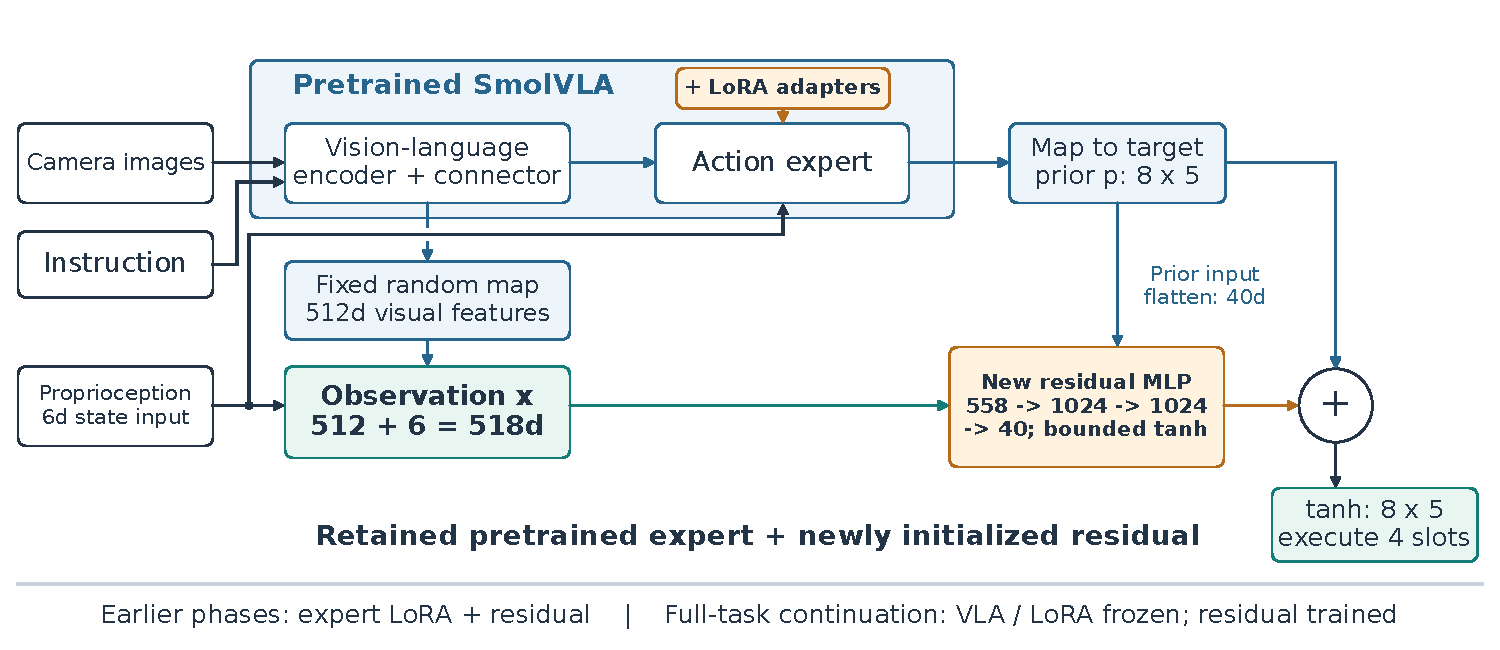
\includegraphics[width=\textwidth]{figures/smolvla_residual_lora.pdf}
\caption{SmolVLA implementation of the pipeline. The added residual combines 518 observation features with a 40-dimensional action prior. LoRA adapts the pretrained expert during earlier training; the evaluated full-task continuation freezes the VLA and LoRA weights. Feature and action dimensions refer to the five-channel controller.}
\label{fig:architecture}
\end{figure*}

\subsection{Milestone-Based Full-Task Composition}
After skill consolidation, one policy learns the complete instruction from empty-gripper starts. No external controller switches between specialist policies. Approach, held pickup, and final placement serve as milestones for assigning credit within a rollout.

The main rule is simple: a later placement failure should not remove the local credit for a successful approach or pickup. We compare milestone outcomes within groups of rollouts from the same scene. Actions receive credit for the milestone they contribute to, while full-task success provides an additional preference for completing the chain. A negative completion bonus is suppressed on already achieved approach and pickup milestones. Placement receives its completion credit once.

This rule preserves useful partial behavior while training the remaining task. It controls the assigned credit; it does not prevent interference through shared network parameters.

\subsection{Stabilized Updates and Full-Task Continuation}\label{sec:rl_loss}
We use a clipped group-relative policy loss with entropy regularization:
\begin{equation}
\mathcal L_{\rm RL}=\mathcal L_{\rm clip}-\eta\mathcal H.
\label{eq:rl_loss}
\end{equation}
The clipped loss compares rollouts within each scene group and limits the incentive for large changes in action likelihood. We use separate upper and lower clipping bounds. The entropy term $\mathcal H$, weighted by $\eta$, maintains exploration during manipulation and composition. Together, these choices help keep early updates conservative while successful behavior is still rare.

During skill learning, DAPO-style dynamic sampling filters uninformative groups and collects additional rollout groups within the configured collection budget~\cite{dapo}. With binary rewards, uniform outcomes provide no group-relative contrast. During dense acquisition, filtering instead checks within-group return variation, so partial progress can provide a learning signal before a group contains a successful skill execution.

Milestone rewards alone need not resolve a full-task plateau. Our CDPR continuation retains the learned bounded residual, freezes the inherited VLA and LoRA, and starts a fresh optimizer while preserving the milestone rewards. The key change is to compute likelihoods from the Gaussian commands sampled before clipping, conditioned on the realized exploration offset. For an episode offset $B$ and its phase gate $g_t$, we store $b_t=g_tB$ and sample
\begin{equation}
u_t\sim\mathcal N(\mu_\theta(x_t,p_t)+b_t,\operatorname{diag}\sigma_\theta^2),
\quad a_t=\operatorname{clip}(u_t,-1,1).
\label{eq:latent_action}
\end{equation}
The robot executes $a_t$, while old and new policy likelihoods score the stored $u_t$ conditional on the same $b_t$. This avoids evaluating a Gaussian density at a clipped boundary~\cite{capg}. Conditioning also accounts for the offset persisting across decisions, instead of treating it as independent extra noise at every step. The residual and exploration scale remain trainable. Algorithm~\ref{alg:paper_pipeline} includes this continuation after a composition plateau; Section~\ref{sec:cdpr_results} reports complete-task performance. Self-imitation uses the regression loss in Eq.~\eqref{eq:si_loss}.

\label{sec:dense_method}
To examine intermediate feedback on a standard benchmark, the LIBERO experiment compares terminal-only, phase-only, and combined dense-and-phase rewards. The combined reward uses a manually defined sequence of reach, grasp, lift, move, and place phases, with a hand-specified progress function for each phase.

At each simulator step, the tracker uses object and gripper state to compute progress for the active phase. Reaching progress increases as gripper--object distance decreases; grasping combines proximity with gripper closure and grasp state; lifting uses height gained above the initial object position; transport uses planar object--target distance; placement uses target proximity, release, and environment success. Each progress measure is normalized to the interval from zero to one. For progress $p_t$ and the phase's previous maximum $p_{\rm best}$, the rewarded increment is $\max(p_t-p_{\rm best},0)$. A completion predicate advances the tracker to the next phase and produces a phase bonus. The weighted progress increment and phase bonus are bounded and combined with terminal feedback. The native task-success verifier remains unchanged.

In the phase-only condition, the continuous progress weight is zero, leaving phase-completion bonuses and terminal feedback.

The dense construction requires a progress function, normalization, and relevant state variables for every phase. Extending it to a new multi-stage task therefore requires further task-specific reward design. This motivates our use of dense feedback for initial skill acquisition and binary milestones for composition: the latter require completion predicates without a continuous progress function for every part of the instruction.

\section{Why Intermediate Feedback Helps}\label{sec:theory}
For $G$ independent candidates from one scene, each with binary success probability $p$, the probability of a mixed-outcome group is
\begin{equation}
P_{\rm mixed}=1-p^G-(1-p)^G.
\label{eq:mixed}
\end{equation}
At $G=8$, it is 21.6\% for $p=0.03$ and 94.2\% for $p=0.30$. Milestones can therefore provide contrast before full success becomes common. Dense progress can distinguish candidates within one milestone level. Neither guarantees useful learning if the feedback is constant or the collector rejects the group.

With separate Bernoulli gates and raw on-policy ascent, suppressing negative completion credit on achieved gates makes each gate's update nonnegative. This finite-model property does not extend directly to a shared neural controller, PPO clipping, or optimizer momentum. We use it to explain the credit rule, without claiming monotonic improvement~\cite{trpo}.

